\section{Overfit\/Underflow}
\begin{frame}
\center \huge \scshape Overfitting
\end{frame}

\begin{frame}
\center
\textbf{Example:}
\\
We want to learn the model that generated some training data:\\
\begin{table}[h]
\begin{tabular}{c}
\multicolumn{1}{l}{\textbf{Training data}} \\ \hline
\multicolumn{1}{|c|}{2135}    \\ \hline
\multicolumn{1}{|c|}{4313}    \\ \hline
\multicolumn{1}{|c|}{1325}    \\ \hline
\multicolumn{1}{|c|}{2213}    \\ \hline
\multicolumn{1}{|c|}{4133}    \\ \hline
\end{tabular}
\end{table}
\end{frame}

\begin{frame}
\begin{table}[h]
\begin{tabular}{c}
\multicolumn{1}{l}{\textbf{Learned model}} \\ \hline
\multicolumn{1}{|c|}{2135}    \\ \hline
\multicolumn{1}{|c|}{4313}    \\ \hline
\multicolumn{1}{|c|}{2135}    \\ \hline
\multicolumn{1}{|c|}{2213}    \\ \hline
\multicolumn{1}{|c|}{4133}    \\ \hline
\end{tabular}
\end{table}
\end{frame}

\begin{frame}
\begin{table}[h]
\begin{tabular}{c}
\multicolumn{1}{l}{\textbf{Learned model $\lambda$}} \\ \hline
\multicolumn{1}{|c|}{2, 2135}    \\ \hline
\multicolumn{1}{|c|}{1, 4313}    \\ \hline
\multicolumn{1}{|c|}{1, 2213}    \\ \hline
\multicolumn{1}{|c|}{1, 4133}    \\ \hline
\end{tabular}
\end{table}
\center
Likelihood of training data: $\prod\limits_O P(O | \lambda)$
\end{frame}

\begin{frame}
What about other data generated by the model?
\begin{table}[h]
\begin{tabular}{cc}
\textbf{New sequences}     & \multicolumn{1}{l}{\textbf{Learned model}} \\ \hline
\multicolumn{1}{|c|}{4135} & \multicolumn{1}{c|}{2, 2135}                  \\ \hline
\multicolumn{1}{|c|}{1322} & \multicolumn{1}{c|}{1, 4313}                  \\ \hline
\multicolumn{1}{|c|}{4213} & \multicolumn{1}{c|}{1, 2213}                  \\ \hline
\multicolumn{1}{|c|}{5135} & \multicolumn{1}{c|}{1, 4133}                  \\ \hline
\multicolumn{1}{|c|}{1345} & 	\multicolumn{1}{c|}{}						                \\ \hline
\end{tabular}
\end{table}
LL of new data?
\begin{itemize}
\item $0$?
\end{itemize}
\end{frame}

\begin{frame}
When does overfitting happen?
\\
\begin{itemize}
\item Learning a too complex model
	\begin{itemize}
	\item Models all the noise
	\end{itemize}
\item Training data too little
	\begin{itemize}
	\item May not reflect model good enough
	\end{itemize}
\end{itemize}
\end{frame}

\begin{frame}
\center
Assume a very general pattern exists:\\
\vspace{20pt}
\begin{tabular}{c}
\multicolumn{1}{l}{\textbf{Training data}} \\ \hline
\multicolumn{1}{|c|}{2\underline{13}5}    \\ \hline
\multicolumn{1}{|c|}{43\underline{13}}    \\ \hline
\multicolumn{1}{|c|}{\underline{13}25}    \\ \hline
\multicolumn{1}{|c|}{22\underline{13}}    \\ \hline
\multicolumn{1}{|c|}{4\underline{13}3}    \\ \hline
\end{tabular}
\end{frame}

\begin{frame}
\center
$1$ always followed by $3$:
\begin{figure}
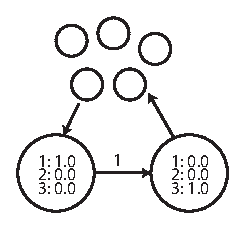
\includegraphics[width=0.45\textwidth]{images/simplemodel.eps}
\end{figure}
\textbf{When learning a simple model:}
\begin{itemize}
\item Cannot express all noise
\item May benefit more from describing general patterns
\end{itemize}
\end{frame}

\begin{frame}
\center
\begin{figure}
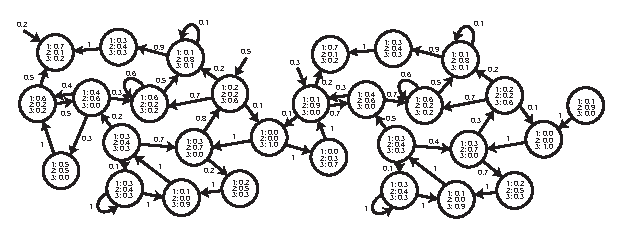
\includegraphics[width=1\textwidth]{images/complexmodel.eps}
\end{figure}
\vspace{40pt}
\textbf{When learning a complex model:}\\
\begin{itemize}
\item May be able to describe all noise
  \begin{itemize}
  \item So why not do it?
  \end{itemize}
\end{itemize}
\end{frame}

\begin{frame}
\center
How do we compare models / algorithms?
\begin{figure}
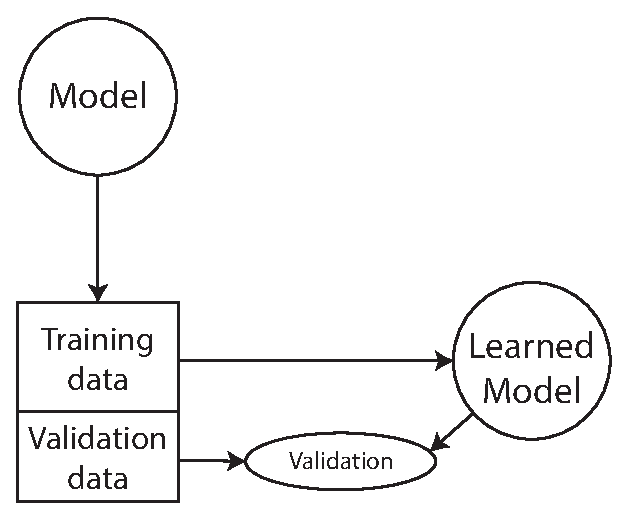
\includegraphics[width=0.7\textwidth]{images/validationdata.eps}
\end{figure}
\end{frame}

\begin{frame}
\center \huge \scshape Avoiding underflow
\end{frame}

\begin{frame}
\center
$P(X) = p_1p_2p_3p_4p_5p_6p_7p_8p_9\cdots$\\
\vspace{20pt}
$0 < p_x < 1$\\
\vspace{20pt}
Underflow when $P(X) = 0$

\end{frame}

\begin{frame}
Visual Studio, C\#: Double precision floating point
\begin{itemize}
\item $0.01^{200} = 0$
\item $0.02^{200} = 0$
\end{itemize}
Probability of a particular sequence can be very small:
\begin{itemize}
\item 23 symbols, uniformly distributed: $\frac{1}{23}^{238} = 0$
\item What about rare symbols?
\item What about probability of 1000 sequences?
\end{itemize}
\end{frame}

\begin{frame}
\center
Solution: Convert to log-space\\
$log \; (a \cdot b) = log \; a + log \; b$\\
\vspace{20pt}
Since $a < b \iff log \; a < log \; b$:\\
\vspace{20pt} 
We can often stay in Log-space
\end{frame}

\begin{frame}
\center
$log (0.01^{200}) = log \; 0.01 + log \; 0.01 + \cdots = -921.034$\\
\vspace{20pt}
$log (0.02^{200}) = log \; 0.02 + log \; 0.02 + \cdots = --782.405$
\end{frame}

\begin{frame}
\center
Problem: How do we sum probabilities in log space?
\end{frame}

\begin{frame}
\center
Problem: How do we sum probabilities in log space?\\
\vspace{20pt}
Solution: Scaling
\end{frame}

\begin{frame}
\begin{table}[h]
\begin{tabular}{|c|l|l|l|l|}
 \hline
Sequence      & 1     & 3    & 3     & 2      \\ \hline
$\alpha_1(i)$          & 0.15  & 0.02 & 0.005 & 0.0007 \\ \hline
$\alpha_2(i)$          & 0.05  & 0.01 & 0.003 & 0.0005 \\ \hline
$\alpha_3(i)$          & 0.2   & 0.02 & 0.01  & 0.003  \\ \hline
\end{tabular}
\end{table}
\end{frame}

\begin{frame}[noframenumbering]
\begin{table}[h]
\begin{tabular}{|c|l|l|l|l|}
 \hline
Sequence      & 1     & 3    & 3     & 2      \\ \hline
$\ddot{\alpha}_1(i)$          & 0.15  & 0.02 & 0.005 & 0.0007 \\ \hline
$\ddot{\alpha}_2(i)$          & 0.05  & 0.01 & 0.003 & 0.0005 \\ \hline
$\ddot{\alpha}_3(i)$          & 0.2   & 0.02 & 0.01  & 0.003  \\ \hline
Sum            & 0.4   &      &       &        \\ \hline
Scaling factor & 2.5   &      &       &        \\ \hline
$\hat{\alpha}_1(i)$          & 0.375 &      &       &        \\ \hline
$\hat{\alpha}_2(i)$          & 0.125 &      &       &        \\ \hline
$\hat{\alpha}_3(i)$          & 0.5   &      &       &        \\ \hline
\end{tabular}
\end{table}
\end{frame}

\begin{frame}[noframenumbering]
\begin{table}[h]
\begin{tabular}{|c|l|l|l|l|}
 \hline
Sequence      & 1              & 3              & 3     & 2      \\ \hline
$\ddot{\alpha}_1$(i)          & 0.15           & \textbf{0.05}  & 0.005 & 0.0007 \\ \hline
$\ddot{\alpha}_2$(i)          & 0.05           & \textbf{0.025} & 0.003 & 0.0005 \\ \hline
$\ddot{\alpha}_3$(i)          & 0.2            & \textbf{0.05}  & 0.01  & 0.003  \\ \hline
Sum            & 0.4            & 0.125          &       &        \\ \hline
Scaling factor & 2.5            & 8              &       &        \\ \hline
$\hat{\alpha}_1(i)$          & \textbf{0.375} & 0.4            &       &        \\ \hline
$\hat{\alpha}_2(i)$          & \textbf{0.125} & 0.2            &       &        \\ \hline
$\hat{\alpha}_3(i)$          & \textbf{0.5}   & 0.4            &       &        \\ \hline
\end{tabular}
\end{table}
\end{frame}

\begin{frame}[noframenumbering]
\begin{table}[h]
\begin{tabular}{|c|l|l|l|l|}
 \hline
Sequence      & 1     & 3            & 3             & 2      \\ \hline
$\ddot{\alpha}_1(i)$          & 0.15  & 0.05         & \textbf{0.32} & 0.0007 \\ \hline
$\ddot{\alpha}_2(i)$          & 0.05  & 0.025        & \textbf{0.2}  & 0.0005 \\ \hline
$\ddot{\alpha}_3(i)$          & 0.2   & 0.05         & \textbf{0.01} & 0.003  \\ \hline
Sum            & 0.4   & 0.125        & 0.53          &        \\ \hline
Scaling factor & 2.5   & 8            & 1.89          &        \\ \hline
$\hat{\alpha}_1(i)$          & 0.375 & \textbf{0.4} & 0.604         &        \\ \hline
$\hat{\alpha}_2(i)$          & 0.125 & \textbf{0.2} & 0.378         &        \\ \hline
$\hat{\alpha}_3(i)$          & 0.5   & \textbf{0.4} & 0.018         &   	   \\ \hline    
\end{tabular}
\end{table}
\end{frame}

\begin{frame}[noframenumbering]
\begin{table}[h]
\begin{tabular}{|c|l|l|l|l|}
\hline
Sequence      & 1     & 3     & 3              & 2                 \\ \hline
$\ddot{\alpha}_1(i)$          & 0.15  & 0.05  & 0.32           & \textbf{0.001323} \\ \hline
$\ddot{\alpha}_2(i)$          & 0.05  & 0.025 & 0.2            & \textbf{0.000945} \\ \hline
$\ddot{\alpha}_3(i)$          & 0.2   & 0.05  & 0.01           & \textbf{0.00567}  \\ \hline
Sum            & 0.4   & 0.125 & 0.53           & 0.007938          \\ \hline
Scaling factor & 2.5   & 8     & 1.89           & 125.98            \\ \hline
$\hat{\alpha}_1(i)$          & 0.375 & 0.4   & \textbf{0.604} & 0.167             \\ \hline
$\hat{\alpha}_2(i)$          & 0.125 & 0.2   & \textbf{0.378} & 0.119             \\ \hline
$\hat{\alpha}_3(i)$          & 0.5   & 0.4   & \textbf{0.018} & 0.714             \\ \hline  
\end{tabular}
\end{table}
\end{frame}